%Talk given virtually for Dagstuhl 2021
\documentclass[11pt,compress,xcolor={usenames,dvipsnames},aspectratio=169]{beamer}
%\documentclass[xcolor={usenames,dvipsnames},aspectratio=169]{beamer} %slides and 
%notes
\usepackage{amsmath,
	amssymb,
	datetime,
	mathtools,
	bbm,
	%mathabx,
	array,
	booktabs,
	xspace,
	multirow,
	calc,
	colortbl,
	siunitx,
 	graphicx}
\usepackage[usenames]{xcolor}
\usepackage[giveninits=false,backend=biber,style=nature, maxcitenames =10, mincitenames=9,mincrossrefs=10]{biblatex}
\addbibresource{FJHown23.bib}
\addbibresource{FJH23.bib}
\usepackage{newpxtext}
\usepackage[euler-digits,euler-hat-accent]{eulervm}
%\usepackage{media9}
%\usepackage[autolinebreaks]{mcode}
\usepackage[tikz]{mdframed}
\usepackage{multicol}

\usepackage{listings}
\definecolor{darkgreen}{rgb}{0,0.6,0}
\lstdefinestyle{Python}{
	%xleftmargin = -1.7in,
	showstringspaces=false,
	language        = Python,
	basicstyle      = \small\ttfamily,
	morekeywords = {as},
	keywordstyle    = \color{blue},
	stringstyle     = \color{darkgreen},
	commentstyle    = \color{darkgreen}\ttfamily,
	breaklines = true,
	postbreak=\text{$\hookrightarrow$\space},
	% style >>> and ... 
	%   see: https://tex.stackexchange.com/questions/326655/make-a-keyword-in-listings-enviorment
	alsoletter = {>,.} ,
	morekeywords = [2]{>>>,...},
	keywordstyle = [2]\color{cyan}\bfseries}


\usetheme{FJHSlimNoFoot169}
\setlength{\parskip}{2ex}
\setlength{\arraycolsep}{0.5ex}

\DeclareMathOperator{\sol}{SOL}
\DeclareMathOperator{\app}{APP}
\DeclareMathOperator{\alg}{ALG}
\DeclareMathOperator{\ACQ}{ACQ}
\DeclareMathOperator{\ERR}{err}
\DeclareMathOperator{\COST}{COST}
\DeclareMathOperator{\COMP}{COMP}
\newcommand{\dataN}{\bigl(\hf(\vk_i)\bigr)_{i=1}^n}
\newcommand{\dataNj}{\bigl(\hf(\vk_i)\bigr)_{i=1}^{n_j}}
\newcommand{\dataNjd}{\bigl(\hf(\vk_i)\bigr)_{i=1}^{n_{j^\dagger}}}
\newcommand{\ERRN}{\ERR\bigl(\dataN,n\bigr)}

\newcommand{\Sapp}{S_{\textup{app}}}
\newcommand{\LambdaStd}{\Lambda^{\textup{std}}}
\newcommand{\LambdaSer}{\Lambda^{\textup{ser}}}
\newcommand{\LambdaAll}{\Lambda^{\textup{all}}}
\newcommand{\oton}{1\!:\!n}
\newcommand{\talert}[1]{\alert{\text{#1}}}
\DeclareMathOperator{\init}{init}
\DeclareMathOperator{\GP}{\cg\cp}
\newcommand{\MLE}{\textup{EB}}
\newcommand{\mCtheta}{{\mathsf{C}_{\vtheta}}}
\newcommand{\mCInv}{\mathsf{C}^{-1}}

%\DeclareMathOperator{\app}{app}

\providecommand{\HickernellFJ}{H.\xspace}


\iffalse
Bayesian cubature proceeds by constructing  credible intervals for the integral based on a prior distribution for the integrand combined with sampled integrand values.  We explain this approach has been developed using low discrepancy (digital net and lattice) sampling and matching covariance kernels to expedite the computation to be much faster than $\Order(n^3)$, where $n$ is the sample size.  We tune the hyper-parameters of our covariance kernels using function data to increase the chance that the integrand is not an outlier. We also show how we have implemented these Bayesian cubature algorithms in QMCPy, a community supported Python library for quasi-Monte Carlo calculations.  Some preliminary results also call into question the Bayesian assumption.  This matter requires further study.
\fi

\renewcommand{\OffTitleLength}{-7ex}
\setlength{\FJHThankYouMessageOffset}{-8ex}
\title{Bayesian Cubature with Low Discrepancy Sequences in QMCPy}
\author[]{Fred J. Hickernell, Jagadeeswaran Rathinavel, \& Aleksei Sorokin}
\institute{Department of Applied Mathematics \qquad
	Center for Interdisciplinary Scientific Computation \\  Illinois Institute of Technology \quad
	\href{mailto:hickernell@iit.edu}{\url{hickernell@iit.edu}} \quad
	\href{http://mypages.iit.edu/~hickernell}{\url{mypages.iit.edu/~hickernell}}}

\thanksnote{Thanks to the GAIL and QMCPy teams \\
	Thanks to the organizers, especially during these unusual times \\
	Disclosure: I am multicultural (computational mathematician \& statistician)\\[2ex]
	Slides at  \href{https://speakerdeck.com/fjhickernell/dagstuhl-bayesian-cubature-ld-qmcpy}{\nolinkurl{speakerdeck.com/fjhickernell/dagstuhl-bayesian-cubature-ld-qmcpy}}}

\event{Probabilistic Numerics @ Dagstuhl}
\date[]{October 27, 2021}

\input FJHDef.tex


\newlength{\figwidth}
\setlength{\figwidth}{0.25\textwidth}

\newlength{\figwidthSmall}
\setlength{\figwidthSmall}{0.2\textwidth}

\newcommand{\financePict}{\href{http://i2.cdn.turner.com/money/dam/assets/130611131918-chicago-board-options-exchange-1024x576.jpg}{\includegraphics[width
		= 3cm]{ProgramsImages/130611131918-chicago-board-options-exchange-1024x576.jpg}}}
	
	\newcommand{\scoop}[1]{\parbox{#1}{\includegraphics[width=#1]{IceCreamScoop.eps}}\xspace}
	\newcommand{\smallscoop}{\scoop{1cm}}
	\newcommand{\medscoop}{\scoop{1.8cm}}
	\newcommand{\largescoop}{\scoop{3cm}}
	\newcommand{\ICcone}[1]{\parbox{#1}{\includegraphics[width=#1,angle=270]{MediumWaffleCone.eps}}\xspace}
	\newcommand{\medcone}{\ICcone{1.2cm}}
	\newcommand{\largercone}{\parbox{2.2cm}{\vspace*{-0.2cm}\includegraphics[width=1cm,angle=270]{MediumWaffleCone.eps}}\xspace}
	\newcommand{\largecone}{\ICcone{1.8cm}}
	\newcommand{\smallcone}{\parbox{1.1cm}{\includegraphics[width=0.5cm,angle=270]{MediumWaffleCone.eps}}\xspace}

	

\newcommand{\northeaststuff}[3]{
	\begin{tikzpicture}[remember picture, overlay]
	\node [shift={(-#1 cm,-#2 cm)}]  at (current page.north east){#3};
	\end{tikzpicture}}


\begin{document}
	\tikzstyle{every picture}+=[remember picture]
	\everymath{\displaystyle}

\frame{\titlepage}

\section{Introduction}

\begin{frame}{Our take on Bayesian Cubature \cite{HicJag18b,RatHic19a,Jag19a,JagHic22a}}
	
	\vspace{-5ex}
		\[
	\mu :=  \int_{[0,1]^d} f(\vx) \, \dif \vx, \qquad \hmu_n = \text{function of } f(\vx_1),  \ldots, f(\vx_n), \qquad \Prob[\abs{\mu - \mu_n} \le \varepsilon] \ge 99\% 
	\]
	
	\begin{itemize}
		\item Assume $f \sim \GP(m,s^2 C_\vtheta)$
		\item<3-> \alert<3>{Choose $C_\vtheta$ and $\vx_1, \vx_2, \ldots$ for a fast eigenvector-eigenvalue decomposition of the Gram matrix $\mC_\vtheta = \bigl(C_\vtheta(\vx_i, \vx_j)\bigr)_{i,j=1}^n$}; this is a \alert<3>{practical} choice, rather than informed by $f$  (see also Kanagawa, Sh\"afer, Wenger)
		\item Sample $f$ at $\vx_1, \ldots, \vx_n$
		\item<2-> \alert<2>{Tune the hyperparameters by empirical Bayes so that $f$ is not an outlier}
		\item Construct a credible interval for $\mu$ in terms of the posterior mean $\hmu_n$
		\item Increase $n$ until the half-width is no greater than $\varepsilon$
		\item<4-> \alert<4>{Implement in software:  GAIL \cite{ChoEtal21a} and QMCPy \cite{QMCPy2020a}} (see also Naslidynk, Pleiss, ProbNum)
	\end{itemize}
	
\end{frame}

\section{Matched Data Sites \& Covariance Kernels}

\begin{frame}{Low Discrepancy (LD) Sequences}
	
\vspace{-3ex}
	
\only<1>{IID sequences have \alert{clusters and gaps}
	
	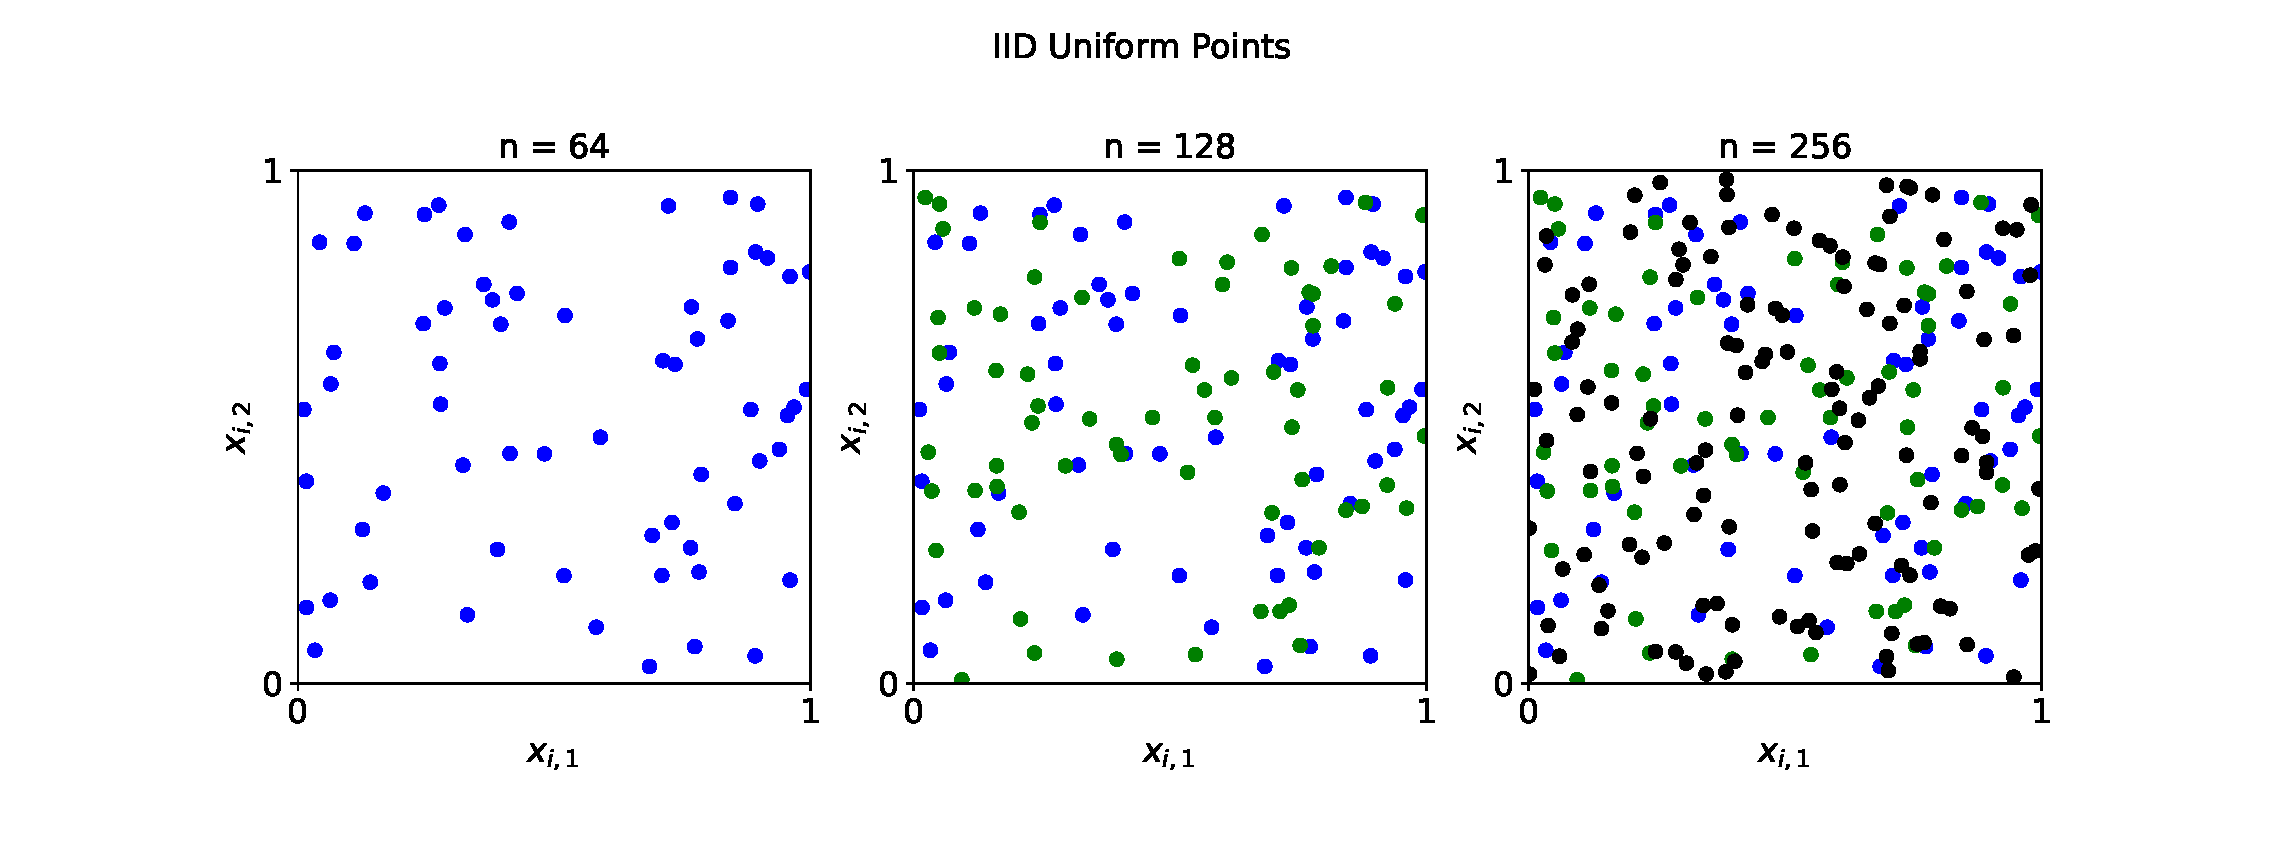
\includegraphics[width = \textwidth]{figures/dd_IID_Uniform.eps}
}
\only<2>{LD lattice sequences are more even than IID
	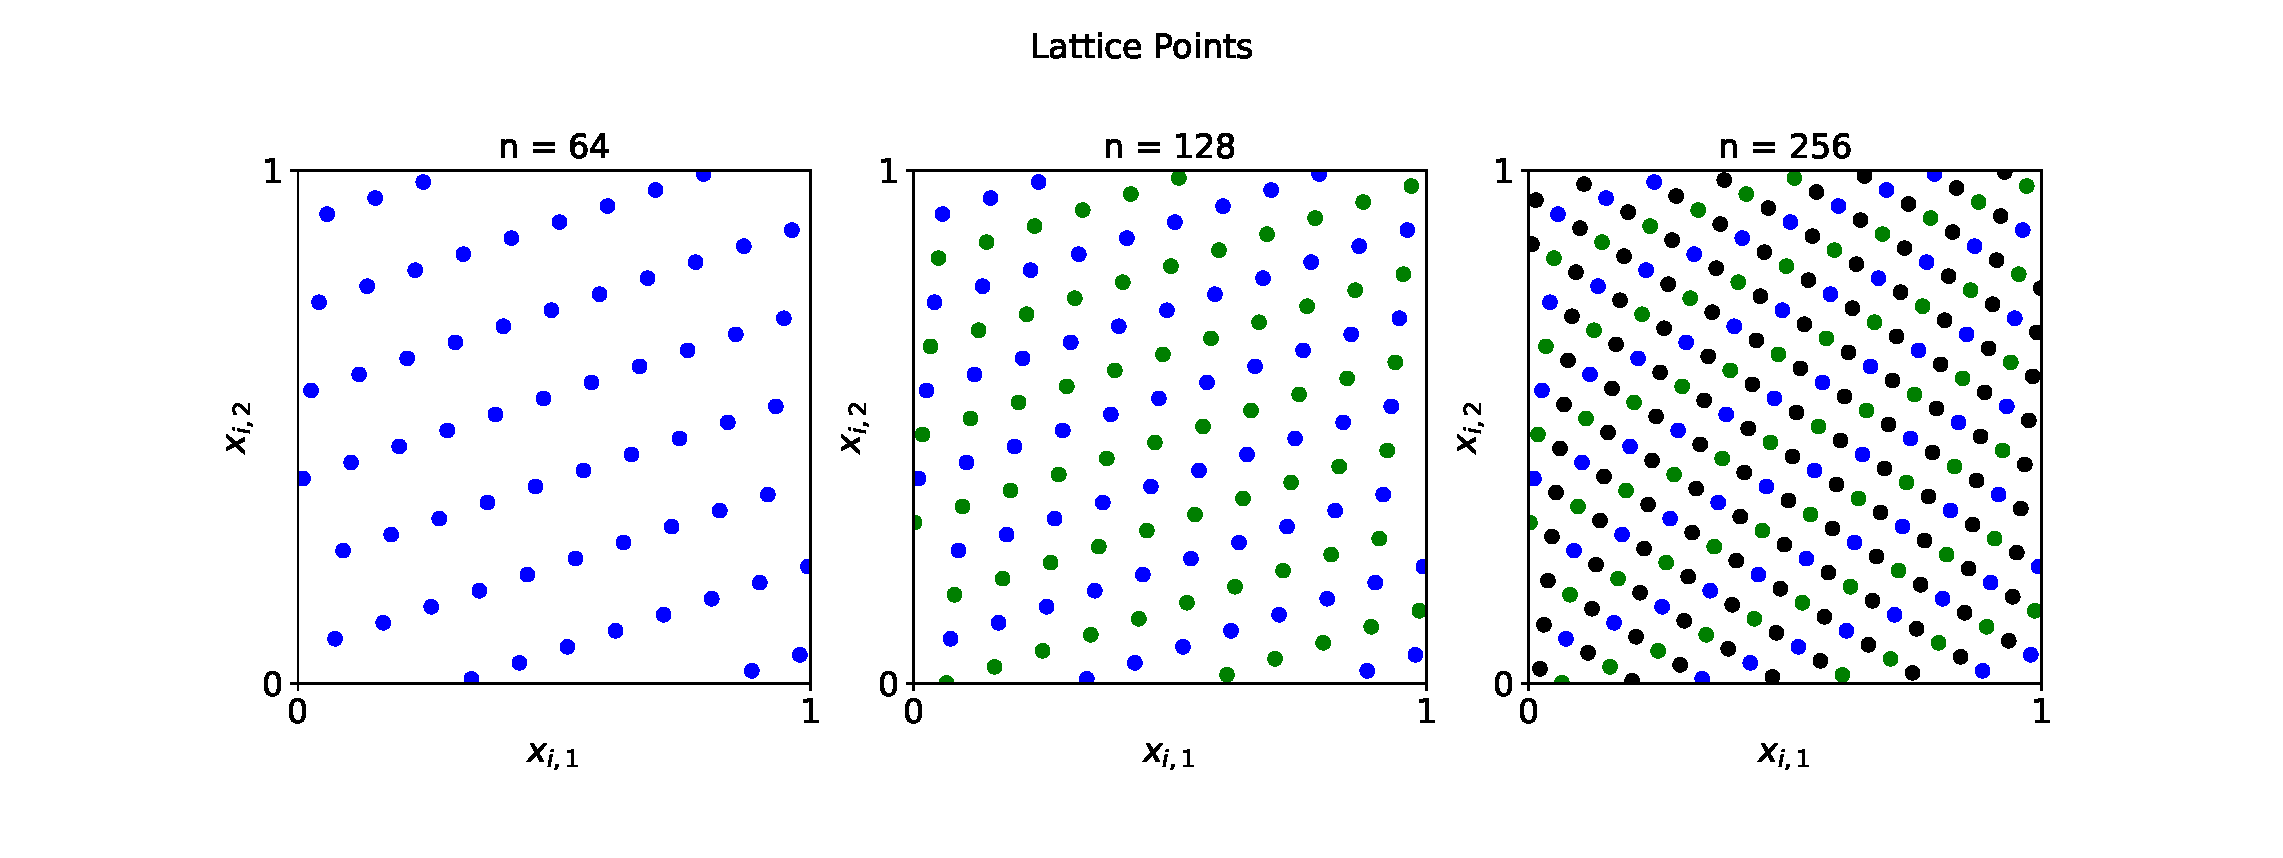
\includegraphics[width = \textwidth]{figures/dd_Lattice.eps}
	
	\vspace{-7ex}
\[
C_\vtheta(\vt,\vx) = K_\vtheta(\vt - \vx \bmod \vone), \qquad \text{e.g., }K(\vt) = \prod_{k=1}^d\bigl[ 1  +  \eta_k  (-1)^{r+1} \underbrace{B_{2r}(t_k)}_{\substack{\text{Bernoulli}\\ \text{polynomial}}} \bigr], \quad \vtheta = (r,\veta)
\]	
}
\only<3>{LD digital sequences (such as Sobol') are more even than IID
	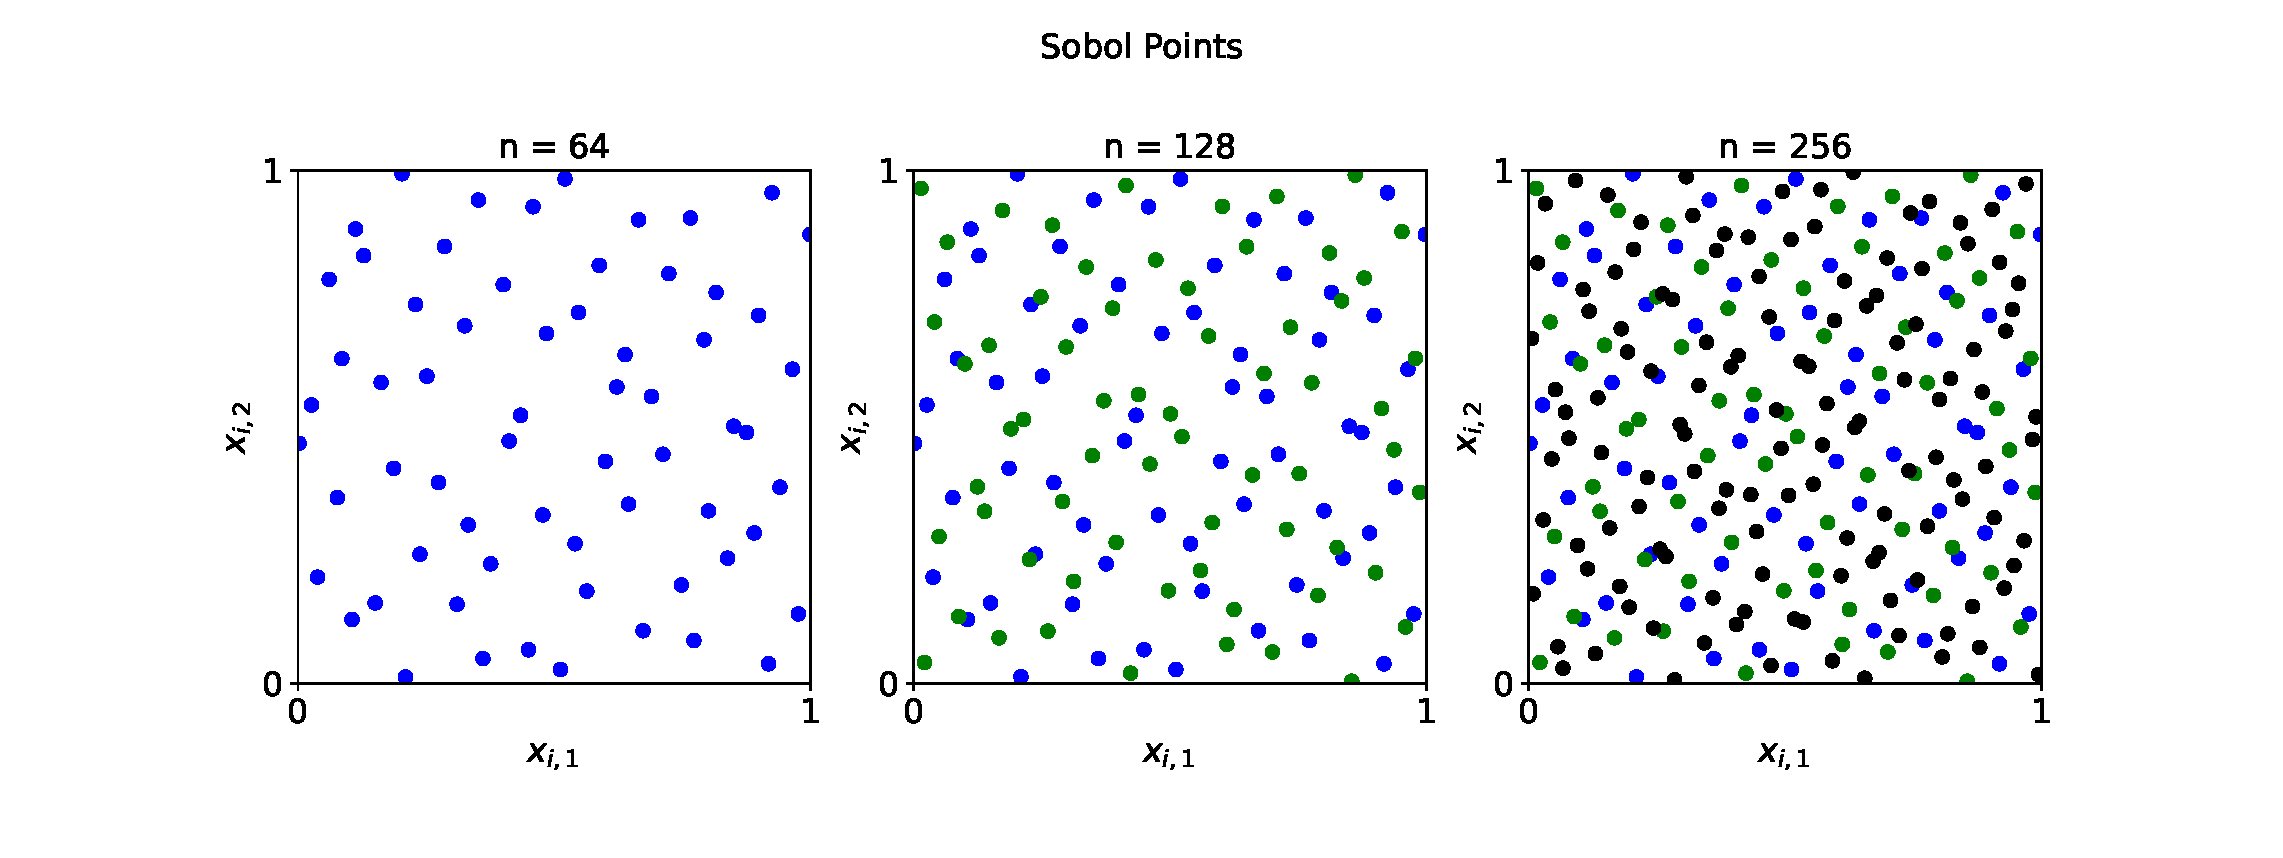
\includegraphics[width = \textwidth]{figures/dd_Sobol.eps}
	
	\vspace{-7ex}
	\[
	C_\vtheta(\vt,\vx) = K_\vtheta(\vt \underbrace{\ominus}_{\substack{\text{digitwise}\\ \text{subtraction}}} \vx ), \qquad \text{e.g., }K(\vt) = \prod_{k=1}^d\bigl[ 1+ \eta_k \underbrace{\omega(t_k)}_{\text{explicit}}\bigr], \quad \vtheta = (r,\veta)
	\]	
}

\end{frame}

\begin{frame}{\only<1>{Eigenvector-Eigenvalue Decomposition of the Gram Matrix}\only<2->{Tuning Hyperparameters and the Credible Interval}}
	For these matched data sites and covariance kernels
	\begin{gather*}
		\only<1-2>{\int_{[0,1]^d} C_\vtheta(\vt,\vx) \, \dif \vt = 1 \quad \forall \vx \in [0,1]^d, \qquad
		\mC_\vtheta = \bigl(C_\vtheta(\vx_i, \vx_j)\bigr)_{i,j=1}^n= \bigl( \vC_{\vtheta 1}, \ldots, \vC_{\vtheta n}) =\frac 1n  \mV \mLambda_\vtheta \mV^H\\
	  \mV \text{ \alert{explict}, (complex exponential or Hadamard)}, \qquad \vV_1 = \vone \\}
	  \vb \mapsto \tvb := \mV^H \vb \text{ is \alert{FFT/FHWT} } \Order (n \log n), \qquad \vlambda_\vtheta := \diag(\mLambda_\vtheta) = \mV^H \vC_{\vtheta 1}, 
	\end{gather*} 
\uncover<2->{which leads to the approximation and credible interval:
\begin{gather*}
	\hmu = \ty_1 = \frac 1n \sum_{i=1}^n f(\vx_i) = \text{sample mean of function values}, \qquad \vy = \bigl(f(\vx_1), \ldots, f(\vx_n) \bigr)^T \\
\Prob \bigl [\abs{\mu - \hmu} \le \ERR\bigr ] = 99\%,  \qquad 
\ERR = \frac{2.58}{n} \sqrt{ \sum_{i = \alert{2}}^n \frac{\lvert \ty_i \rvert^2}{\lambda_{\vtheta i}} \left(1 - \frac{n}{\lambda_{\vtheta 1}} \right)} 
\only<3>{ \\
\vtheta_{\text{opt}} =  \argmin_{\vtheta} \left [ \log \left( \sum_{i=\alert{2}} \frac{\lvert \ty_i \rvert^2}{\lambda_{\vtheta i}}\right)   + \frac 1n \sum_{i=1}^n \log(\lambda_{\vtheta i} )  \right ]
}
\end{gather*}
}

\end{frame}
	
\section{QMCPy}

\begin{frame}{Our Methods Bayesian Stopping Criteria into Software}
	
	\vspace{-3ex}
	
	Our research on stopping criteria (Bayesian and otherwise) has been implemented in two libraries:
	\begin{itemize}
		\item GAIL \cite{ChoEtal21a} MATLAB library (born in 2013)
		\item QMCPy \cite{QMCPy2020a} Python library (born in2019)
	\end{itemize}
Our goals are to provide software that 
\begin{itemize}
	\item Includes the best (mostly QMC) algorithms available
	\item Is well-tested
	\item Is easy to use, gives practitioners an easy on-ramp
	\item Provides use cases for algorithm developers 
	\item Plays well with other packages
\end{itemize}
	
	
\end{frame}
	

\begin{frame}[fragile]\frametitle{Keister Example in QMCPy}
	\vspace{-5ex}
	\[
	\mu = \int_{\reals^d} \cos(\norm{\vt}) \exp(-\norm{\vt}^2) \, \dif \vt = \int_{[0,1]^d} f(\vx) \; \dif \vx =  ? \qquad \text{Keister \cite{Kei96}}
	\]
\noindent\begin{minipage}{0.47\textwidth}
\begin{lstlisting}[style=Python]
d = 5; tol = 1e-2
lattice = Lattice(dimension=d, order='linear')
integrand = Keister(lattice)
solution,data = CubBayesLatticeG(integrand, abs_tol=tol, ptransform = 'none').integrate()
print(data)
\end{lstlisting}
\end{minipage} 
\qquad
\begin{minipage}{0.47\textwidth}
\begin{lstlisting}[style=Python]
solution        1.136
error_bound     0.009
n_total         1024
time_integrate  0.725
abs_tol         0.010
rel_tol         0
n_init          2^(8)
n_max           2^(22)
\end{lstlisting}
\end{minipage} 

\end{frame}


\begin{frame}[fragile]\frametitle{Asian Option Pricing Example in QMCPy}
	\vspace{-5ex}
	\[
	\text{option price} = \mu = \int_{\reals^d} \text{payoff}(\vz) \; \text{discrete BM PDF}(\vz)   \, \dif \vz = \int_{[0,1]^d} f(\vx) \; \dif \vx  = ? \quad \text{Glasserman  \cite{Gla03}}
	\]
\noindent\begin{minipage}{0.52\textwidth}
\begin{lstlisting}[style=Python]
volatility=.5; interest_rate =.01
start_price = 30; strike_price = 25
t_final = 1; call_put = 'call'
mean_type = 'arithmetic'
d = 4; abs_tol = .01
integrand = AsianOption(Lattice(d, order = 'linear'), volatility, start_price, strike_price, interest_rate, t_final, call_put, mean_type)
solution,data = CubBayesLatticeG(integrand,abs_tol=abs_tol).integrate()
print(data)
\end{lstlisting}
\end{minipage} 
\qquad
\begin{minipage}{0.42\textwidth}
\begin{lstlisting}[style=Python]
solution        6.235
error_bound     0.007
n_total         2048
time_integrate  1.470
abs_tol         0.010
rel_tol         0
time_vec        [0.25 0.5  0.75 1.  ]
covariance      [[0.25 0.25 0.25 0.25]
[0.25 0.5  0.5  0.5 ]
[0.25 0.5  0.75 0.75]
[0.25 0.5  0.75 1.  ]]
decomp_type     PCA
\end{lstlisting}
\end{minipage} 
	
\end{frame}


\section{Unsolved Challenges}

\begin{frame}[fragile]\frametitle{Slow Speed, Wrong Answers}
{\small 
\vspace{-3ex}

Computations \href{https://colab.research.google.com/drive/1KrlrtLu7j8Ff7YsSJjPMiGUr-UKfqwxm?usp=sharing}{\beamergotobutton{here}}

\vspace{-3ex}
\begin{center}
{\footnotesize
\begin{tabular}{rccccl}
	Example & Stopping Criterion & $d$ & Absolute Tolerance & $n$ & Time \\ \toprule
	Keister & Bayesian Lattice \cite{RatHic19a} & $5$ & $0.01$ & $2^{10}$ & $0.943$ s \\
	Keister & Bayesian Sobol' \cite{JagHic22a} &&&  $2^{12}$ & $0.102$ s \\
	Keister & Track Fourier Coef.\ Lattice \cite{JimHic16a} &&& $2^{13}$ & $0.024$ s \\
	Keister & Track Fourier Coef.\  Sobol' \cite{HicJim16a} &&& $2^{13}$ & $0.012$ s \\ \midrule
	Keister & Bayesian Lattice \cite{RatHic19a} & $5$ & $0.001$ &  & \alert{$> 10$ m} \\
	Keister & Track Fourier Coef.\ Lattice \cite{JimHic16a} &&& $2^{17}$ & $0.388$ s \\ \toprule
Option Pricing  & Bayesian Lattice \cite{RatHic19a} & $4$ & $0.01$ & $2^{10}$ & $1.347$ s \\
Option Pricing  & Track Fourier Coef.\ Lattice \cite{JimHic16a} &&& $2^{12}$ & $0.021$ s \\ \midrule
Option Pricing  & Bayesian Lattice \cite{RatHic19a} & $13$ & $0.01$ & \multicolumn{2}{c}{\alert{wrong answer}}\\
Option Pricing  & Track Fourier Coef.\ Lattice \cite{JimHic16a} &&& $2^{12}$ & $0.034$ s \\ \bottomrule
\end{tabular}
}
\end{center}
\vspace{-3ex}
\begin{itemize}
	\setlength{\itemsep}{-0.5ex}
	\item Computational load in \alert{optimizing} for the kernel parameters
	\item \alert{Inefficient} code
	\item The speed may not be a problem if function evaluation is \alert{expensive}
\end{itemize}
}
\end{frame}


\begin{frame}[fragile]\frametitle{Checking the Gaussian Process Assumption}


\end{frame}







\finalthanksnote{These slides are  available at \\  \href{https://speakerdeck.com/fjhickernell/dagstuhl-bayesian-cubature-ld-qmcpy}{\nolinkurl{speakerdeck.com/fjhickernell/dagstuhl-bayesian-cubature-ld-qmcpy}}}


\thankyouframe

\printbibliography

	
\end{document}
\begin{frame}{Quasi-Monte Carlo Cubature}
	
	\vspace{-6ex}
	
	\[
	\uncover<3->{\mu :=  \int_{\ct} \alert<4>{g(\vt)} \, \alert<3>{\lambda(\vt) \, \dif \vt} \underbrace{=}_{\alert<3>{\vt = \vT(\vx)}} } \only<1>{\mu :=} 	\underbrace{\int_{[0,1]^d} \alert<4>{f(\vx)} \, \dif \vx}_{\text{integration}} =  \underbrace{\Ex[f(\vX)]}_{\substack{\text{expectation} \\ \text{population mean}}} \approx  \underbrace{\frac 1{\alert<5>{n}} \sum_{i=1}^{\alert<5>{n}} f(\alert<2>{\vX_i})}_{\text{sample mean}} =: \hmu_{\alert<5>{n}}
	\]
	
	\vspace{-3ex}
	
	\begin{description}[<+(1)->]
		\setlength{\itemsep}{0.5cm}
		
		\item[Low Discrepancy Generators] producing $\vX_1, \vX_2, \dots \LDsim \cu[0,1]^d$
		
		\item[True Measures] $\lambda$ used to define the original integral, such as Lebesgue or Gaussian, along with the variable transformation (importance sampling)
		
		\item[Integrands] $g$ used to define original integral and the final, transformed integrand, $f(\vx) = g(\vT(\vx))\lambda(\vT(\vx))\abs{\vT'(\vx)}$ (preferably flat)
		
		\item[Stopping Criteria] that determines how large $n$ should be to ensure that $\abs{\mu - \hmu_n} \le \varepsilon$
	\end{description}
\end{frame}

\begin{frame}{Software Landscape}
	\vspace{-3ex}
	{\small 
	
	\renewcommand{\arraystretch}{1.15}
	\begin{tabular}{>{\centering}m{0.47\textwidth}@{\qquad}>{\centering}m{0.47\textwidth}}
		\alert{LD Sequence Generators} & \alert{Multi-Level, Stopping Criteria, Applications}
		\tabularnewline \toprule
		\href{https://www.mathworks.com}{\alert{MATLAB}}---Sobol' \& Halton 
		&
		\multirow{2}{0.47\textwidth}{\centering \href{https://people.maths.ox.ac.uk/gilesm/mlmc/}{\alert{Mike Giles}}---Multi-Level (Quasi-)Monte Carlo  in C++, MATLAB, Python, R}
		\tabularnewline
		\href{http://www.broda.co.uk}{\alert{BRODA}---Sobol' in C, MATLAB, and Excel}
		\tabularnewline
		\href{https://Sci.Py.org/}{\alert{SciPy}}, \href{https://pytorch.org/}{\alert{PyTorch}---Sobol', Halton, more in Python}
		&
		\multirow{2}{0.47\textwidth}{\centering \href{http://gailgithub.github.io/GAIL_Dev/}{\alert{Guaranteed Automatic Integration Library (GAIL)}}---Stopping criteria  in MATLAB}
		\tabularnewline
		\href{https://github.com/google/tf-quant-finance}{\alert{Tensorflow}}---Nets, lattices \& finance in Python
		\tabularnewline
		\href{https://cran.r-project.org/web/packages/qrng/qrng.pdf}{\alert{\texttt{qrng}}}--- R package, Sobol' and Halton 
		&
		\multirow{2}{0.47\textwidth}{\centering  \href{https://www.uqlab.com}{\alert{UQLab}}---Framework for Uncertainty Quantification in MATLAB}
		\tabularnewline
		\href{http://statweb.stanford.edu/~owen/code/}{\alert{Art Owen}}---randomized Halton in R  
		\tabularnewline 
		\href{https://github.com/PieterjanRobbe/QMC.jl}{\alert{Pieterjan Robbe}---LD sequences in Julia}
		&
		\multirow{3}{0.47\textwidth}{\centering \href{http://www.openturns.org}{\alert{OpenTURNS}---An Open source initiative for the Treatment of Uncertainties, Risks 'N Statistics in Python}}
		\tabularnewline 
		\href{https://github.com/stevengj/Sobol.jl}{\alert{Steven Johnson}}---Sobol' in Julia 
		\tabularnewline 
		\href{https://developer.nvidia.com/curand}{\alert{cuRAND}}---Sobol' in CUDA
		\tabularnewline
		\multicolumn{2}{>{\centering}m{0.96\textwidth}}{\href{http://simul.iro.umontreal.ca}{\alert{Pierre L'Ecuyer}---LatNet Builder and  Stochastic Simulation in C/C++ and Java}}
		\tabularnewline
		\multicolumn{2}{>{\centering}m{0.96\textwidth}}{\href{https://people.cs.kuleuven.be/~dirk.nuyens/}{\alert{Dirk Nuyens}}---Magic Point Shop and QMC4PDE in MATLAB, Python, and C++}
		\tabularnewline
		\multicolumn{2}{>{\centering}m{0.96\textwidth}}{\href{http://people.sc.fsu.edu/~jburkardt/}{\alert{John Burkhardt}}---variety in C++, Fortran, MATLAB, \& Python}
		\tabularnewline
		\multicolumn{2}{>{\centering}m{0.96\textwidth}}{\href{https://qmcsoftware.github.io/QMCSoftware/}{\alert{QMCPy}}---Python package incorporating and connecting the work of different groups}
		\tabularnewline
	\end{tabular}
	
}
	
	\renewcommand{\arraystretch}{1}
	
\end{frame}

\begin{frame}{What We Want}
\begin{multicols}{2}
	\begin{itemize}
		\item QMC in the hands of more users
		
		\item Quality QMC algorithms
		
		\item Platform to compare performance of competing QMC algorithms
		
		\item Vehicle to explore QMC for new use cases
		
	\end{itemize}
	
	\columnbreak
\includegraphics[width = 0.45\textwidth]{QMCSoftwarePlot.eps}	
\end{multicols}

\end{frame}


\section{Low Discrepancy Generators}

\begin{frame}{Low Discrepancy Generators: $\vX_1, \vX_2, \dots \LDsim \cu[0,1]^d$}
\begin{multicols}{2}
{\Large \alert{Recent Advances}}\\ [-1ex]
\begin{itemize}
	\item \href{https://github.com/scipy/scipy/pull/10844}{\alert{Sobol' and Halton into SciPy.}}  Zeroth point included; discrepancy; transformations to other distributions
	
	\item Lattices, digital nets, and quantitative finance  into \href{https://github.com/google/tf-quant-finance}{\alert{Tensorflow}}
	
	\item Niederreiter points and other ``bring your own'' generators in QMCPy
	
\end{itemize}

\columnbreak
\uncover<2>{
{\Large \alert{Challenges}}\\ [-0.5ex]
\begin{itemize}
	\item Need to educate \href{https://arxiv.org/pdf/2008.08051.pdf}{\alert{against}} dropping, thinning, burn-in, power of $10$ sample sizes \cite{Owe22a}
	
	\item Need to go beyond \alert{$2^{32}$} points
	
	\item \alert{Nested uniform scrambling} of nets \cite{Owe95}, as an alternative to linear matrix scrambling, not yet widely available
	
	\item \alert{Higher order nets} not widely available
	
	\item \alert{Which} generators are significantly better 
	\begin{itemize}
		\item For which practical problems?
		\item For higher dimensions?
	\end{itemize}

\item Is there a useful hybrid of lattices and digital sequences?
\end{itemize}
}

\end{multicols}
\end{frame}

\section{True Measures}

\begin{frame}{True Measures:  $\vT: \ct \to [0,1]^d$ }

\vspace{-8ex}
	\[
\int_{\ct} g(\vt) \, \lambda(\vt) \, \dif \vt \underbrace{=}_{\alert{\vt = \vT(\vx)}} \int_{[0,1]^d} f(\vx) \, \dif \vx \qquad \text{\alert{Variable transformations} aka \alert{importance sampling}}
\]

	\begin{multicols}{2}
		{\Large \alert{Recent Advances}}
		\begin{itemize}
			
			\item SciPy has several 
			
			\item QMCPy has defaults for $\vT = \reals^d$ or $[\va,\vb]^d$ based on  the original weight function, and you can choose your own
						
		\end{itemize}
		
		\columnbreak
		
		\uncover<2>{
		{\Large \alert{Challenges}}
		\begin{itemize}
			\item Importance sampling is an art
			
			\item Need for \href{https://statweb.stanford.edu/~owen/pubtalks/AdaptiveISweb.pdf}{\alert{adaptive importance sampling}}
			
			\item Can some importance sampling make QMC competitive with MCMC for Bayeseian inference, etc. \cite{Zha21a}?
			
			\item Transformations for non-rectangular $\ct$ (simplex, ball, sphere)  not widely available
			
		\end{itemize}
	}
		
	\end{multicols}
\end{frame}

\section{Integrands}

\begin{frame}{Integrands or Use Cases $	\int_{\ct} \alert{g(\vt) \, \lambda(\vt)} \, \dif \vt = \cdots$}
	
	\begin{multicols}{2}
		{\Large \alert{Recent Advances}}
		\begin{itemize}
			
			\item \href{https://github.com/google/tf-quant-finance}{\alert{Tensorflow}} has quantitative finance 
			
			\item UQLab and OpenTURNS include LD generators for their use cases
			
			\item QMCPy allows you to build your own, and has a growing number of examples

			\item New use cases such as in Robbe's talk \cite{Vro19a} on system reliability and Ebert's talk combining QMC with algorithmic differentiation
			
		\end{itemize}
		
		\columnbreak
		
		\uncover<2>{
			{\Large \alert{Challenges}}
			\begin{itemize}
				\item Our go-to use cases need refreshing and expanding
				
				\item Hard to swap out different LD generators for important use cases because the use cases do not have a common interface or is not always accessible
				
				\item Need to demonstrate connecting a package that computes the integrand values (such as an open source PDE solver) with the package that does the QMC
				
			\end{itemize}
		}
		
	\end{multicols}
\end{frame}

	
\section{Stopping Criteria}

\begin{frame}{Stopping Criteria, $n = ?$ to Satisfy Error Tolerance}
	
	\begin{multicols}{2}
		{\Large \alert{Recent Advances}}
		\begin{itemize}
			\item QMCPy includes 
			\begin{itemize}
				\item Several kinds of stopping criteria including replications, tracking Fourier coefficients \cite{HicJim16a,JimHic16a}, and Bayesian credibility intervals \cite{RatHic19a}
				\item Criteria to ensure that $\bigl \lvert \sol - \widehat{\sol}_n \bigr \rvert \le   \max(\varepsilon_{\text{a}}, \varepsilon_{\text{r}} \abs{\sol})$, where
				$\sol$ is a function of more than one integral, e.g., Bayesian inference, Sobol' indices
			\end{itemize}
						
		\end{itemize}
		
		\columnbreak
		
		\uncover<2>{
			{\Large \alert{Challenges}}
			\begin{itemize}
				\item Need better stopping criteria for higher order nets (other than replications)
				
				\item Need better stopping criteria for more complex problems, such as parametric integration, density estimation, Markov Chain Monte Carlo
				
			\end{itemize}
		}
		
	\end{multicols}
\end{frame}

\section{Conclusion}

\begin{frame}{Final Thoughts}
	
\begin{multicols}{2}
	\begin{itemize}
		\item Several multi-collaborator projects are growing in functionality and user base
		
		\item Can our work build a shorter path between research code and production code?

		\item Can our Python packages talk to one another?
		
		\item Do we ignore or encourage development in R, Julia, MATLAB, \ldots?
		
		\item Need to be careful about licensing issues as we share and adapt code
				
	\end{itemize}
	
	\columnbreak
	\includegraphics[width = 0.45\textwidth]{QMCSoftwarePlot.eps}	
\end{multicols}
	
\end{frame}


\finalthanksnote{These slides are  available at \\  \href{https://speakerdeck.com/fjhickernell/advances-and-challenges-in-quasi-monte-carlo-software}{\nolinkurl{speakerdeck.com/fjhickernell/advances-and-challenges-in-quasi-monte-carlo-software}}}


\thankyouframe

\printbibliography


\end{document}





